\subsection{Redpanda}

Redpanda merupakan \textit{event streaming platform}. \textit{Platform} ini menyediakan infrastruktur untuk \textit{streaming real-time data}. \textit{Producers} mengirimkan data berupa \textit{events} ke Redpanda, kemudian Redpanda menyimpan \textit{events} tersebut dan mengaturnya ke dalam sebuah \textit{topic}. \textit{Topic} ini merupakan log perubahan sistem yang dapat diputar ulang. \textit{Consumer} mengonsumsi \textit{events} pada \textit{topic} Redpanda secara asinkron \parencite{redpandaIntro}.

Redpanda merupakan \textit{event streaming platform} alternatif dari Apache Kafka. Selain merupakan alternatif, \textit{platform} ini menawarkan kompatibilitas API yang sama dengan Kafka sehingga memudahkan migrasi penggunanya. Meskipun begitu, terdapat beberapa perbedaan antara Redpanda dengan Apache Kafka.

\begin{figure}[ht]
    \centering
    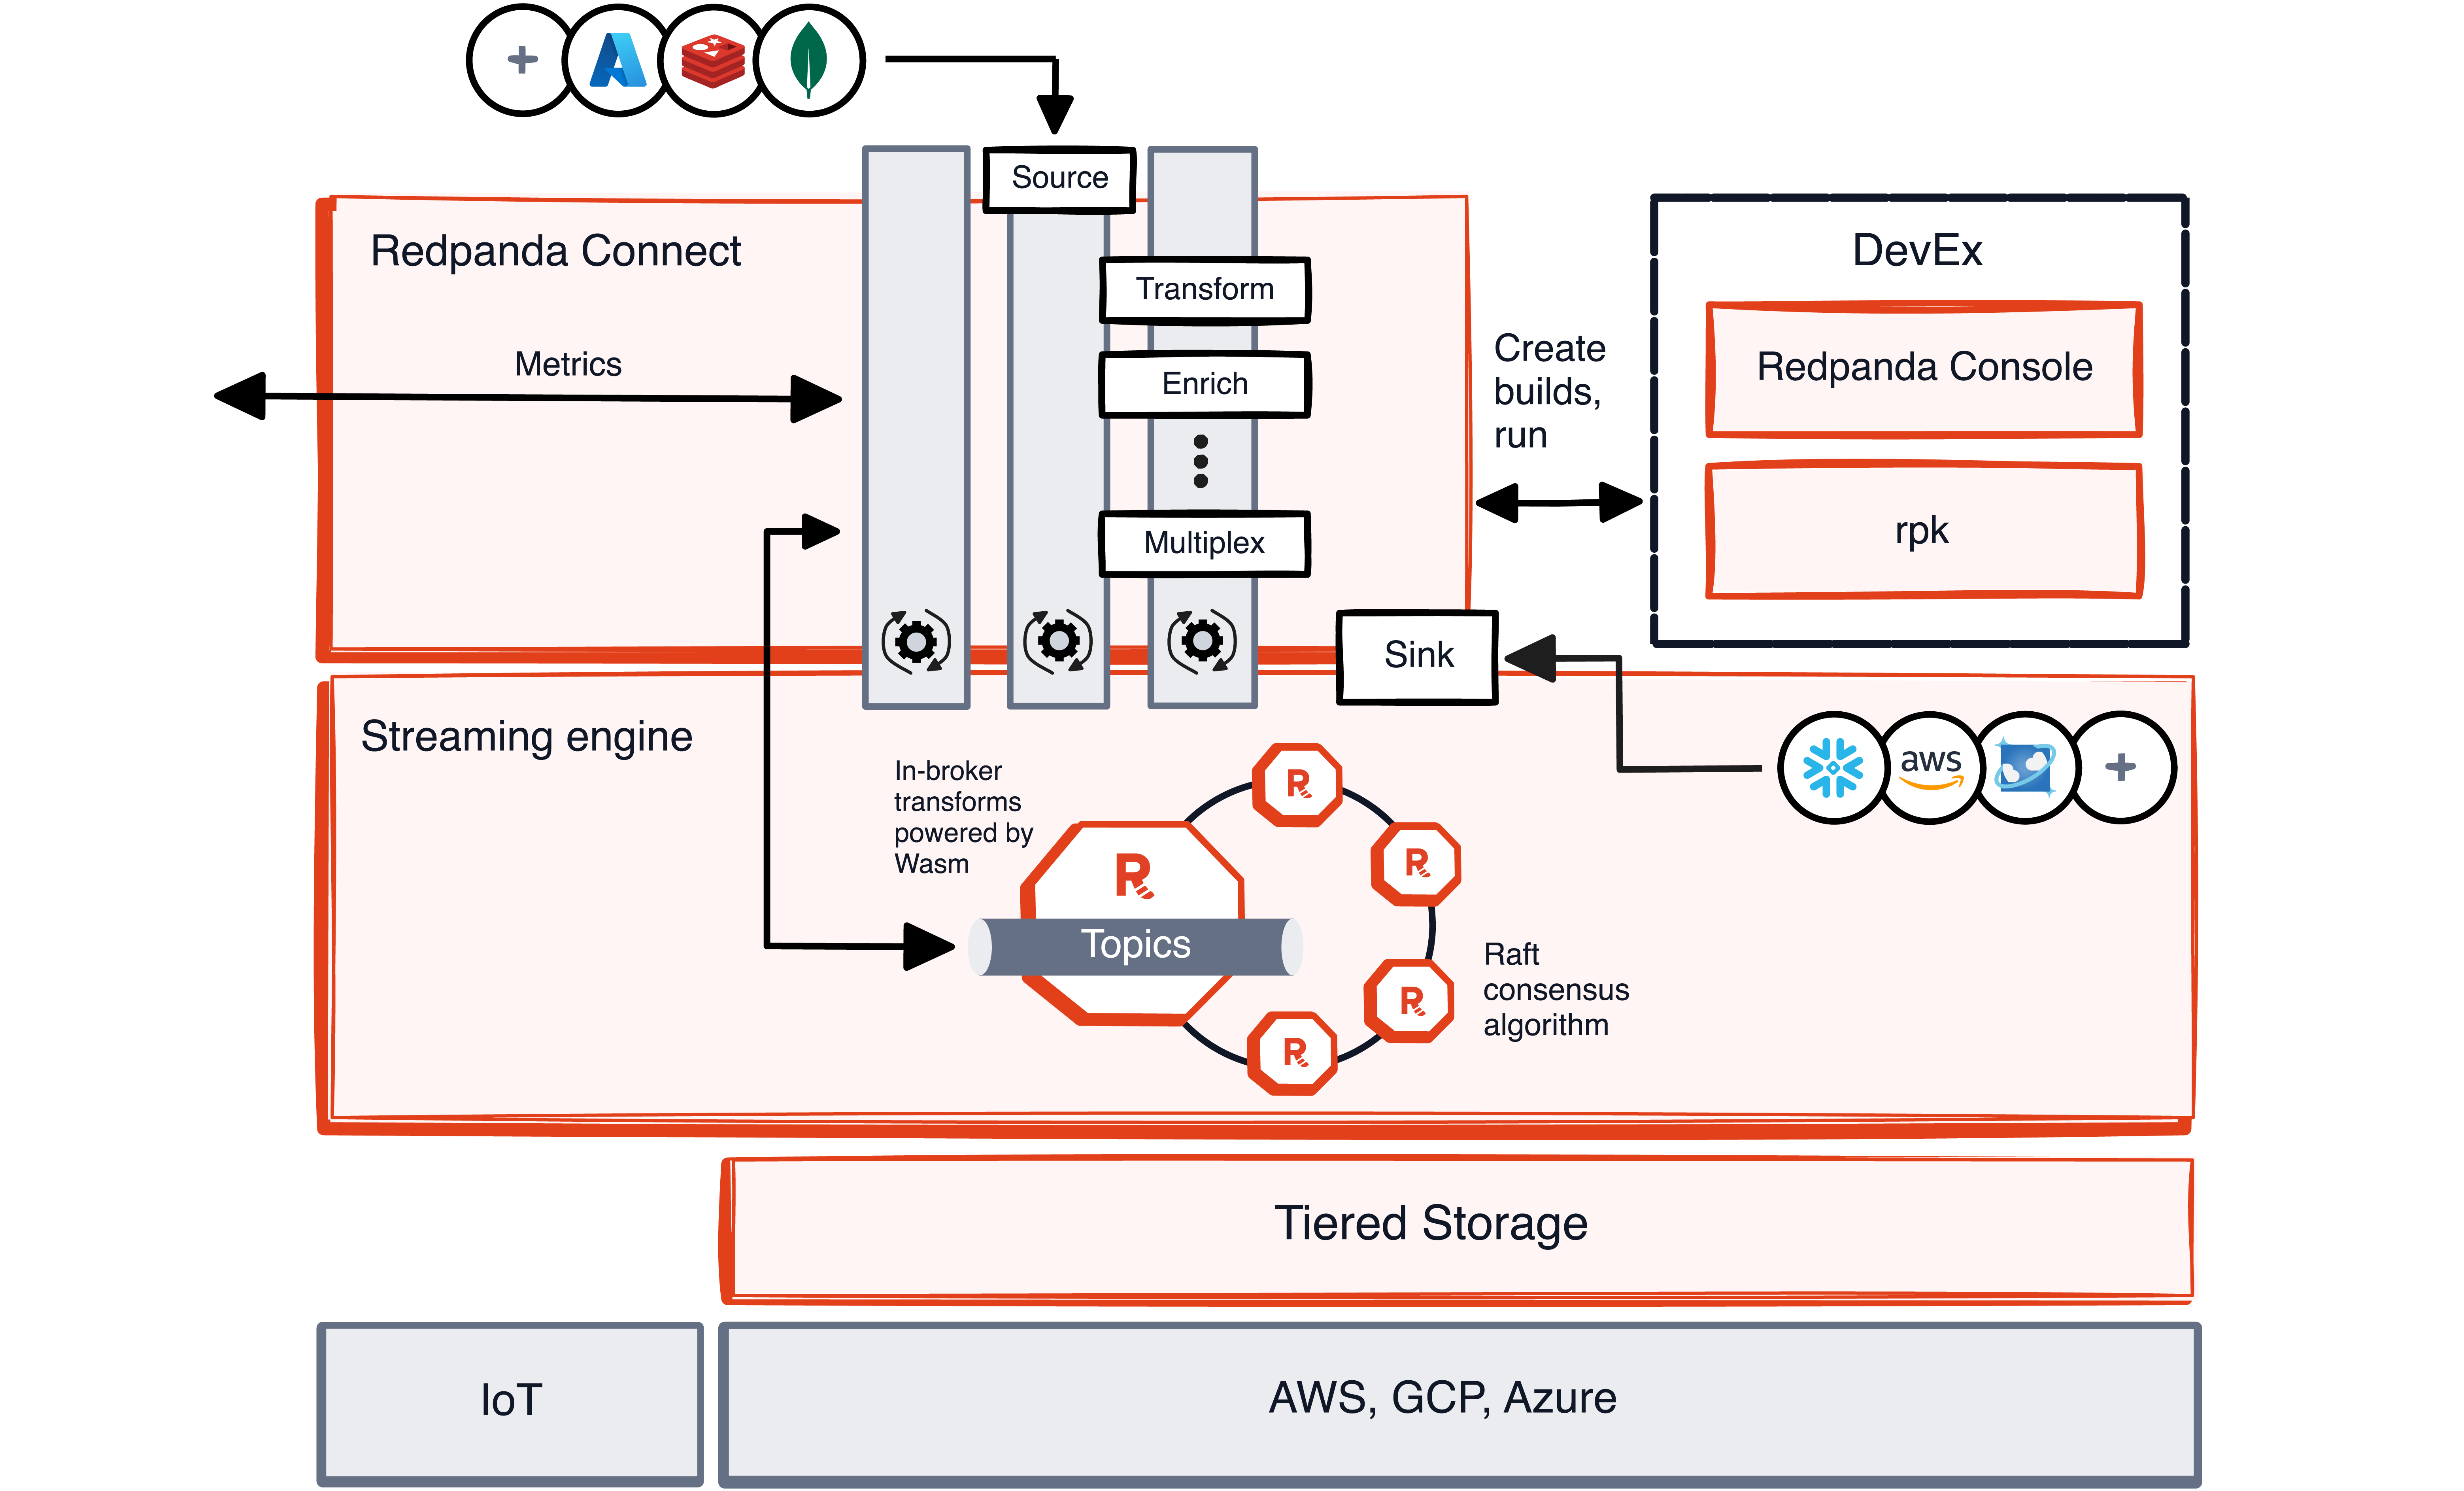
\includegraphics[width=0.8\textwidth]{resources/chapter-2/redpanda.png}
    \caption{\textit{What is Redpanda? \parencite{whatIsRedpanda}}}
    \label{fig:what-is-redpanda}
\end{figure}

Perbedaan pertama adalah algoritma konsensus yang digunakan. Apache Kafka menggunakan ZooKeeper (versi lama) sedangkan Redpanda menggunakan Raft. Meskipun begitu, versi terbaru Kafka sudah menggunakan algoritma konsensus Kraft yang merupakan varian dari Raft dengan perbedaan pada mekanisme \textit{log replication} \parencite{raftKraft}.

Selain itu, Redpanda berfokus pada pengoptimalan kinerja yang lebih baik dibandingkan dengan Apache Kafka. Redpanda ditulis dalam bahasa C++, sedangkan Apache Kafka berjalan pada JVM. Dalam hal ini, Redpanda menggunakan bahasa sistem sehingga minim \textit{overhead}. Berikut adalah contoh pengoptimalan yang dilakukan pada Redpanda: \textit{Direct Memory Access (DMA)} untuk I/O, distribusi pemrosesan \textit{interrupt request} (IRQ) pada beberapa core CPU, penggunaan model \textit{thread per core}, dan lain-lain. Penggunaan model \textit{thread per core} memungkinkan Redpanda untuk menjalankan \textit{thread} aplikasinya pada core CPU yang sama sehingga \textit{context switching} dan \textit{blocking} dapat dihindari \parencite{redpandaArchitecture}.